\chapter{User Enjoyment Improvement}
One of the main goals of Reminisce.me is to get people to play a lot of games in order to be able to collect a lot of information. The more a person plays and the longer they keep coming back to the game the more detailed the analysis can be. It is also important that the users enjoy the game enough for them to talk about it and attract more users. In general, we can say that this project trades enjoyment for data about autobiographical memory. For that to be possible, we need the game to be enjoyable and the player to feel comfortable while playing. A lot of measures have been been put in place to make the whole experiment as good as possible.
\section{Mobile improvements}
Most of the people today access the internet on their mobile device more than they do on a laptop or desktop computer. In fact, the largest part of Facebook users are mobile users \cite{mobileusage}. Therefore, we can safely expect that a decent portion of our user base will be mobile users, playing while on transportation or during a break. Making the experience great for these players is then an important concern.
\subsection{Mobile application: motivations}
Up to now, the way to access Reminisce.me on a mobile device was through a browser on the phone. Some basic application had been tested in the past but it could not really be used as a replacement for the web application. The problems that come from using Reminisce.me on a mobile phone are the following:
\begin{enumerate}
	\item It uses a lot of bandwidth: there is a lot of data downloaded to get to the website, it is rarely a problem when using it with a proper wi-fi or cabled connection but becomes one when using the mobile network
	\item Some features, such as the notifications, the Facebook login and the Facebook friends invitations do not behave correctly or do not work at all.
\end{enumerate}
Building a mobile application solves those problems. With an application installed on the phone, the amount of data the user has to download to play the game is less than on a website as some data is already stored on the phone this way. We can have separate code running on the mobile for specific parts which need a different treatment so we can make all the features work on all platforms.
\subsection{Building a mobile application with Meteor}
Writing a mobile application is a tedious task and requires a lot of development. Fortunately, Meteor comes coupled with Cordova\cite{cordova} which makes the bold promise of enabling developers to create a native mobile application with the fewest possible changes. This works by having most of the application code running in a web view on the mobile (much like an in-application internet browser, but without an address bar) and only have specialized code when you want to use a native functionality (camera, notifications, etc.). Thus, for most of the application we only need to make sure that our design is responsive and works well on small smartphones screens. It also offers the possibility to clearly separate the code which runs on a the Cordova (mobile) platform and the one intended to run anywhere else through a simple boolean check.

\subsection{Future improvements}
We did not manage to provide an iOS version of the application and it is therefore only possible to try it on an Android phone. The first important step would be to make sure that we can provide a proper iOS version of the application before trying to improve it. Most of the work has been done and hopefully it is just a matter of doing a similar work for iOS.\\\\
As far as improvements are concerned, it is important to know that at the moment of writing, the mobile application has the same features as the website and most of them work at a satisfying level. However, in some aspects it still looks a lot like a web page displayed on a mobile phone and some parts of the interface (such as the ordering questions) still need to be improved to provide a better user experience.


\subsection{No post ordering}\label{subsec:postorder}
Displaying the content of a post on a question has always been an issue. The content of posts vary a lot from one to an other. They may contain images, links, videos, text or a combination of multiple of those elements. There is no real limit to the length of a post and it is hard to plan the layout of graphical interface accordingly. This means that it is sometimes necessary to scroll to read the whole post or that the alignment of the objects displayed is suboptimal. On top of this issue, the ordering questions are sometimes hard to handle on a mobile device because the drag and drop movement can be used to either scroll through the question or reorder the items. The combination of those two issues made it impossible to guarantee a nice user experience on the mobile application so it was decided to drop the questions implying to reorder posts.
\section{Blacklist}
Even though some discomfort such as reading old posts from a time when the user was a lot younger and a lot less mature can be funny, we still need to make sure this discomfort does not exceed a certain level. While the application was being tested by different users, some users came across content related to people they did not wish to hear about or events they are not willing to think about.\\\\
There are two main problems with those questions. The first is tied to a person. Be it an ex partner or a dead relative, we all know people whose name suffices to bring back painful memories or sad feelings. While this is a really unfortunate situation and it might diminish our capacity to generate questions, we felt compelled to add the possibility for the user to ignore Facebook users they do not want any mention of on their game boards. The main reason behind this decision is that, depending on the relationship between a potential player and some of the people mentioned in the questions, the discomfort can be big enough for the user to not want to play the game again. Unfortunately, it is impossible for us to predict when such a situation might arise and we cannot do a lot preemptively (beside highlighting the blacklist button so that the user thinks about it before even starting to play), but we hope that having the ability to ignore people is sufficient to make users stay after encountering such a situation. Figure \ref{fig:blacklist} shows the interface where a user can edit its blacklist.\\\\
The second problem is related to a particular event and is linked more to the content of a post than to the a person reacting, commenting or being mentioned in it. This problem is still open at the moment as analyzing the content (text, title or image) to see if it is related to something as abstract as an event is not an easy problem and would require more advanced machine learning techniques.
\begin{figure}
\centering
{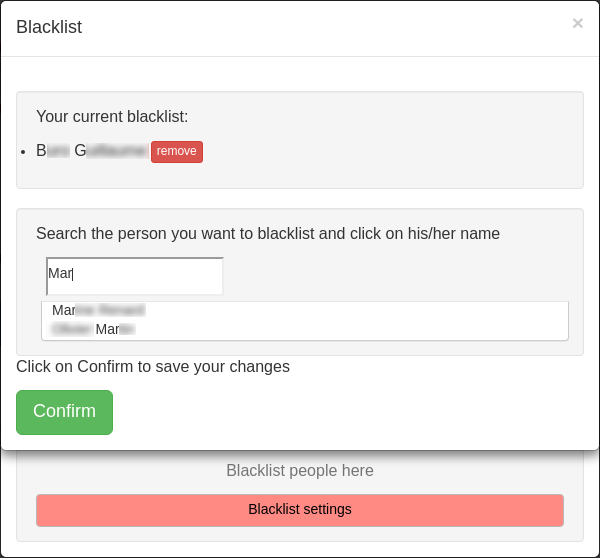
\includegraphics[width=3.5in]{images/blacklist.png}}
\caption{Blacklist Interface}
\label{fig:blacklist}
\end{figure}

\section{Notifications}
As mentioned in the previous thesis, a notification system has been developed to keep the users engaged. During the initial pilot, all of the application's notifications ("Your opponent played a move." and "Someone invited you to play a game.") were forwarded to the social Facebook's notification system. This would generate a large amount of notifications on the social network and it was reported by multiple users as being quite annoying.
Therefore, we decided to follow Facebook's best practices guidelines on notifications \cite{fbappnotif} and only send notifications via Facebook twice a day. This means that twice a day, when you visit the social network, you will receive a summary of the received notifications during the last 12 hours instead of receiving one for each individual event. On the other hand, the notifications are still displayed on the application in two ways: a small black popup on the top right part of the screen and a browser notification \cite{browsernotif} (or a mobile one if it is on a mobile platform).

\section{Displaying statistics to the user}
One of the cool things about playing a game is to measure your performance at the game. People like to be able to quantify their skill level for anything so it felt important to us to provide some statistics to the user. A new page was added with three new sections. We show the overall performance in terms of wins ties and loss (figure \ref{fig:statsWTL}), the performance on each individual question type (in terms of amount of good answers and mean time spent on the question as shown on figure \ref{fig:statsQP}) and the performance over time in terms of wins, ties ans losses. For instance, figure \ref{fig:statsTI} shows that I am not really improving.
\begin{figure}
\centering
{
\includegraphics[width=2in]{images/wtl.png}}
\caption{Statistics page: Win-Tie-Loss}
\label{fig:statsWTL}
\end{figure}
\begin{figure}
\centering
{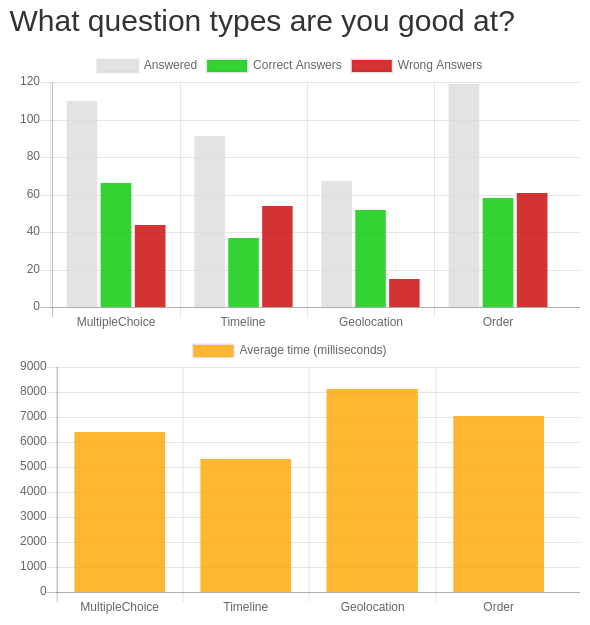
\includegraphics[width=4in]{images/questions_perf.png}}
\caption{Statistics page: performance by question type}
\label{fig:statsQP}
\end{figure}
\begin{figure}
\centering
{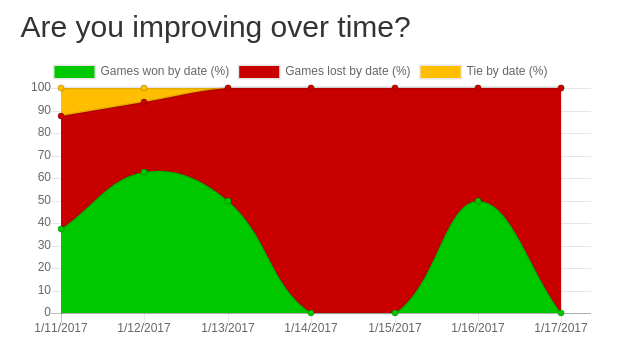
\includegraphics[width=4.5in]{images/time_improv.png}}
\caption{Statistics page: improvement over time}
\label{fig:statsTI}
\end{figure}